\chapter[The LHC and the ATLAS detector][The LHC and the ATLAS detector]{The LHC and the ATLAS detector}
\label{chap:lhcatlas}

\begin{quote}
  The LHC and ATLAS detector are described.
\end{quote}
 
\section{The LHC}
\label{sec:lhc}

\begin{figure}[tp]
  \centering
  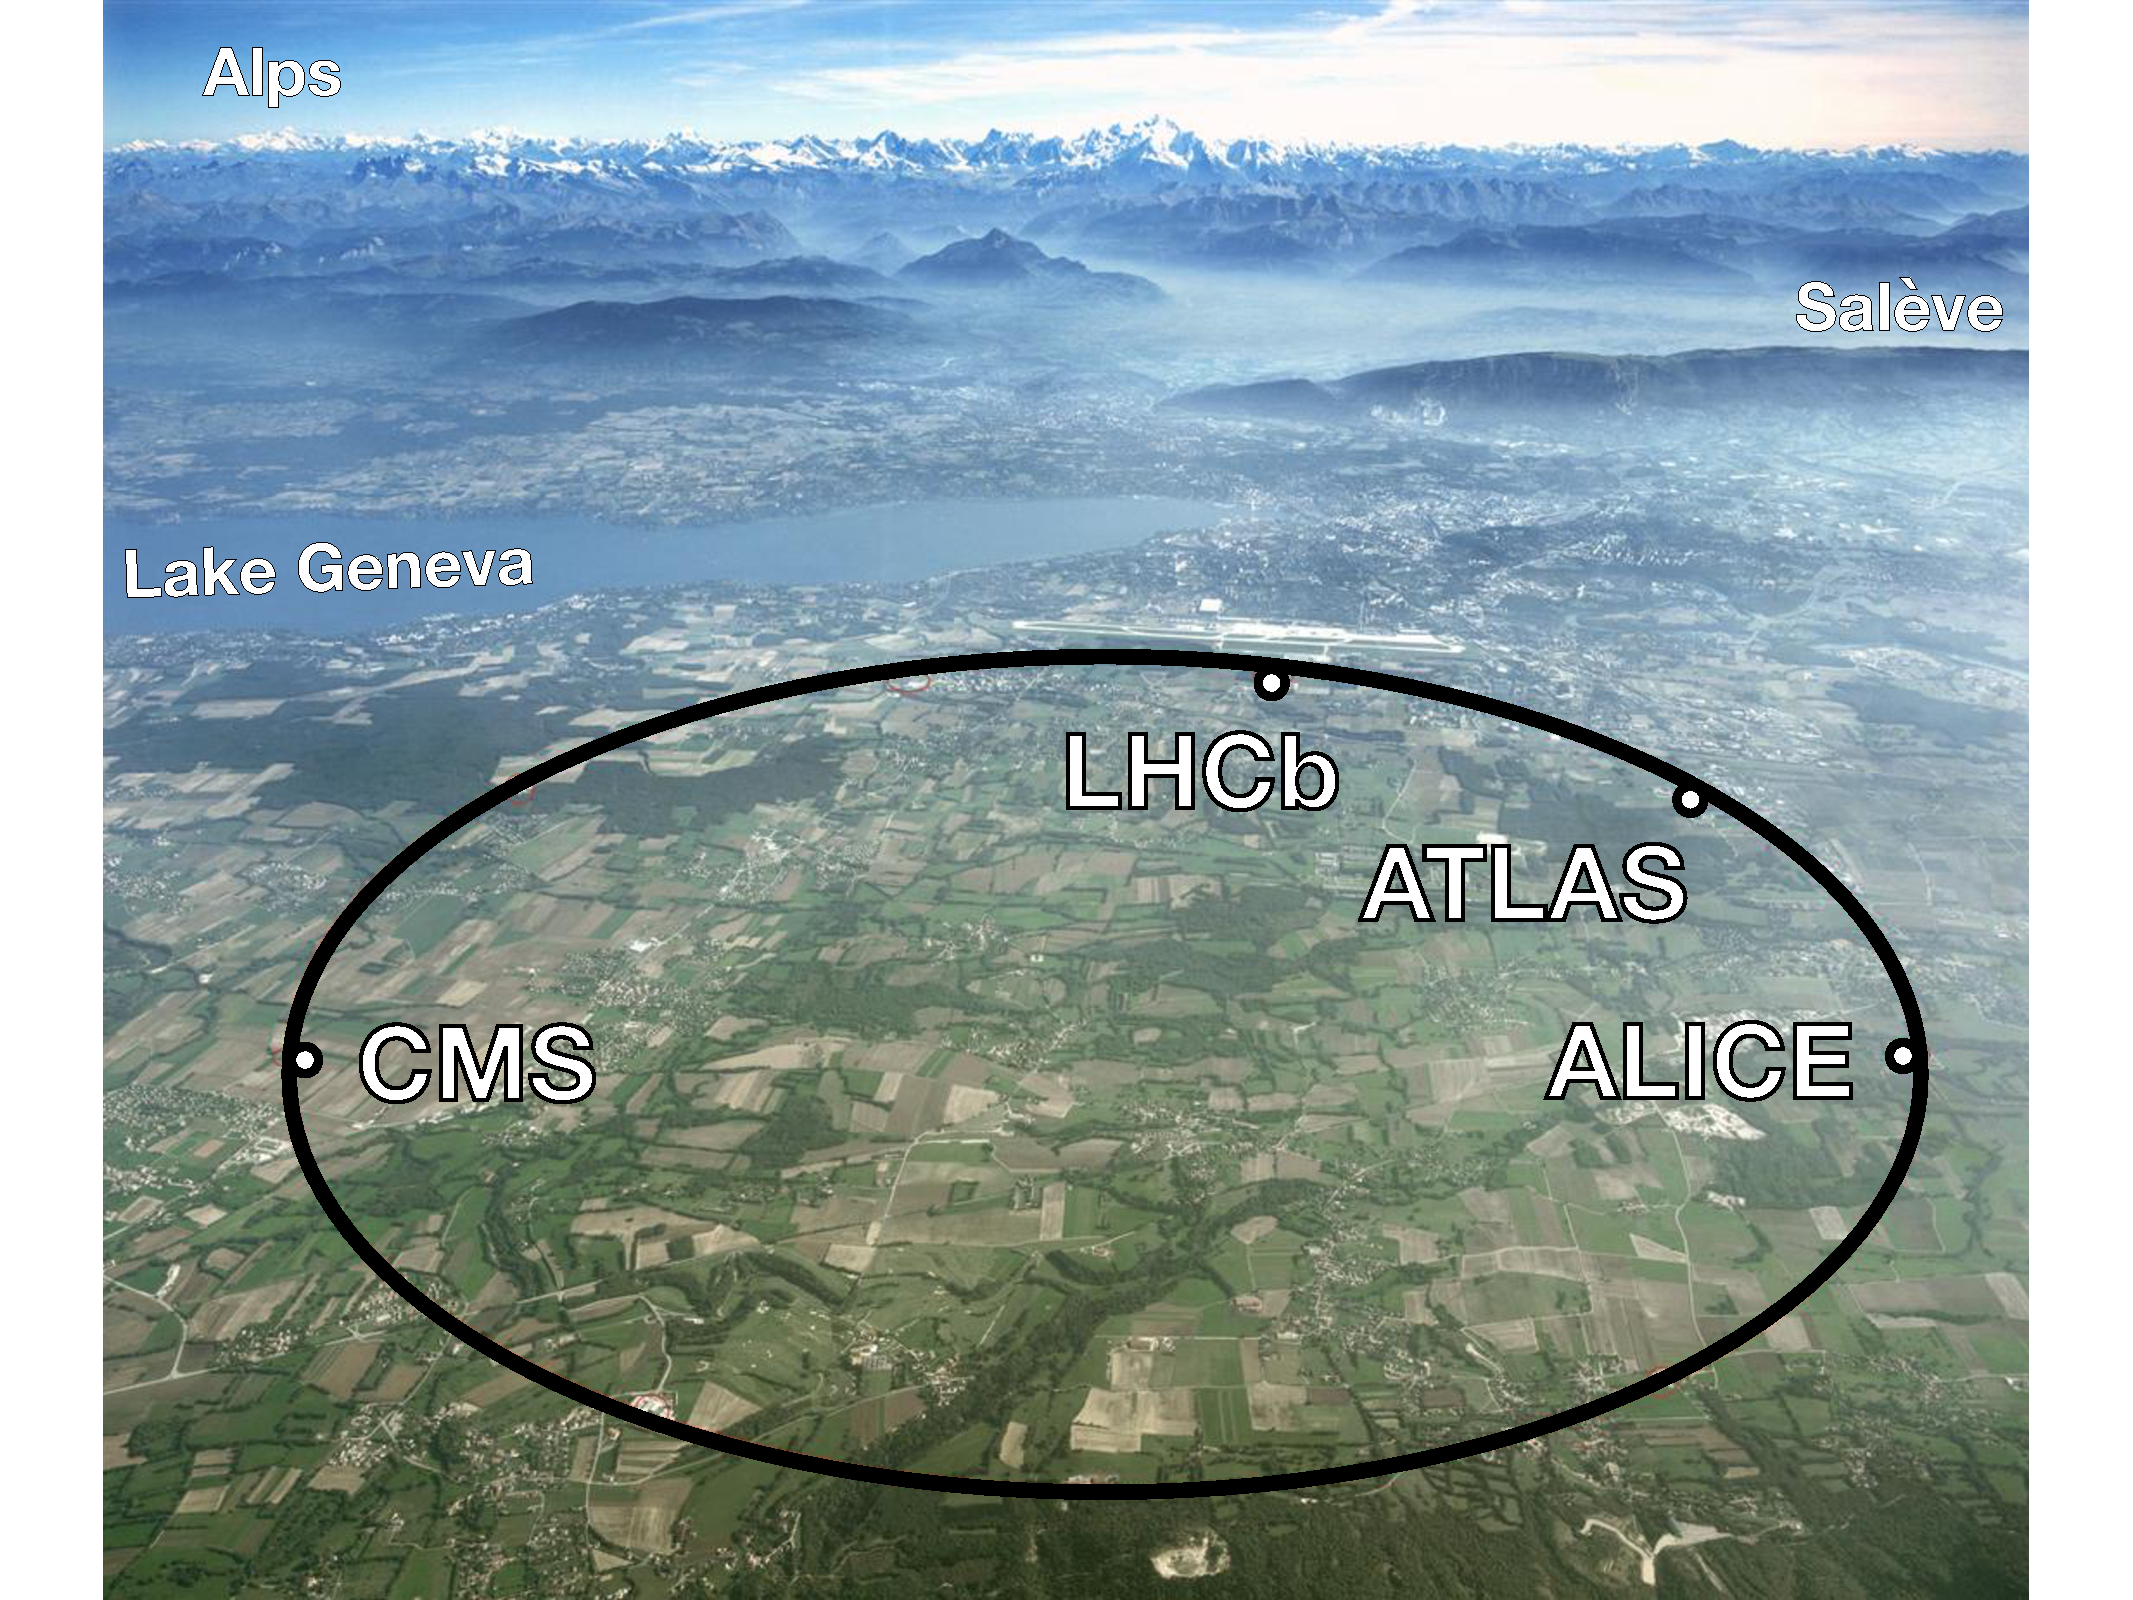
\includegraphics[width=0.90\textwidth]{figures/lhc-atlas/lhc-switzerland}
  \caption{Aerial view of Geneva with an overlaid drawing of the LHC and associated experiments~\cite{atlas-surface}.}
  \label{fig:lhc-switzerland}
\end{figure}

\begin{figure}[tp]
  \centering
  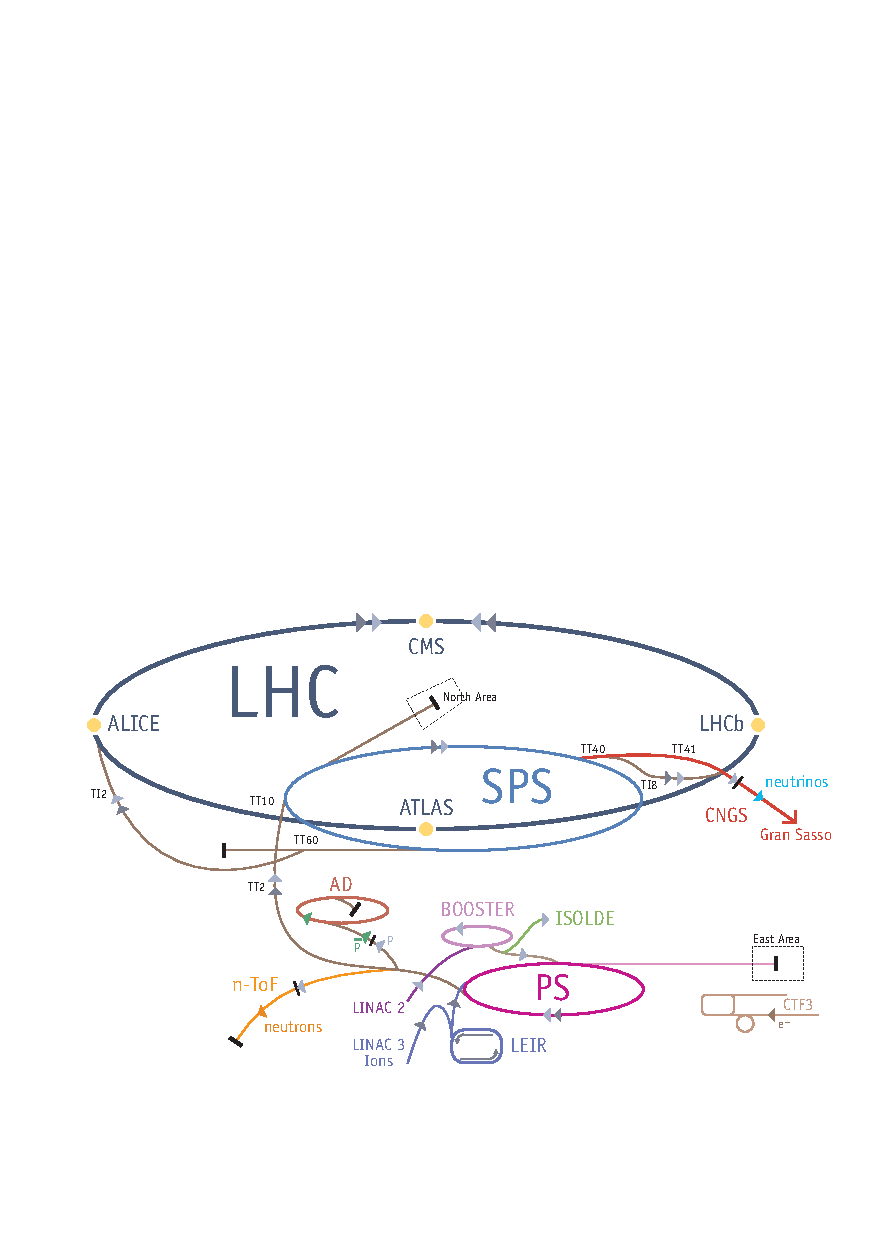
\includegraphics[width=0.90\textwidth]{figures/lhc-atlas/lhc-accelerator-complex}
  \caption{The LHC accelerator complex. Before reaching the LHC, protons are accelerated at Linac 2, the Proton Synchrotron Booster (PSB), the Proton Synchrotron (PS), and the Super Proton Synchrotron (SPS)~\cite{cern-faq}.}
  \label{fig:lhc-complex}
\end{figure}

\begin{figure}[tp]
  \centering
  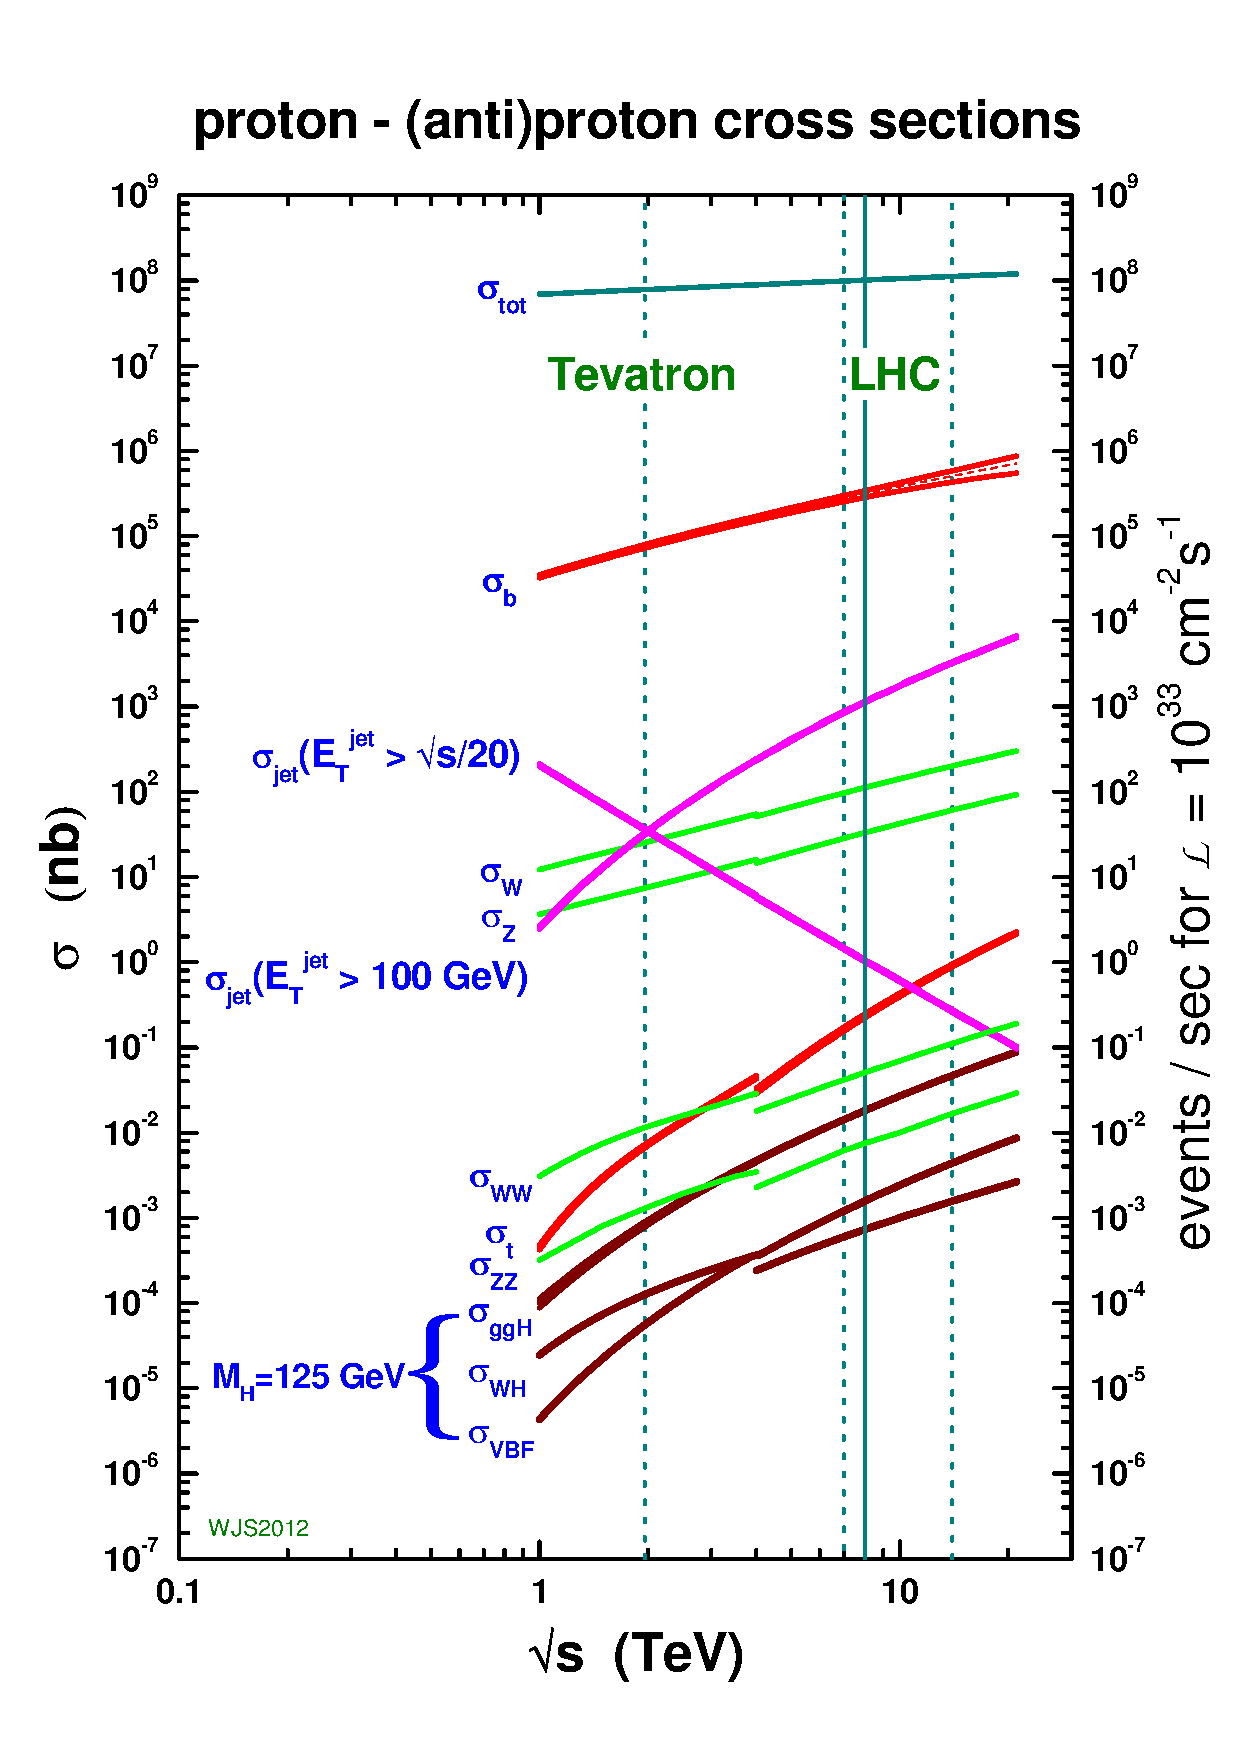
\includegraphics[width=0.90\textwidth]{figures/lhc-atlas/crosssections2012_v5}
  \caption{Cross sections for $pp$ and $p\overline{p}$ processes in the center-of-mass energy regime relevant to the Tevatron and LHC, courtesy of W.J. Stirling~\cite{2013.stirling.cross-sections}.}
  \label{fig:lhc-stirling}
\end{figure}

\section{The ATLAS detector}
\label{sec:atlas}

\begin{figure}[tp]
  \centering
  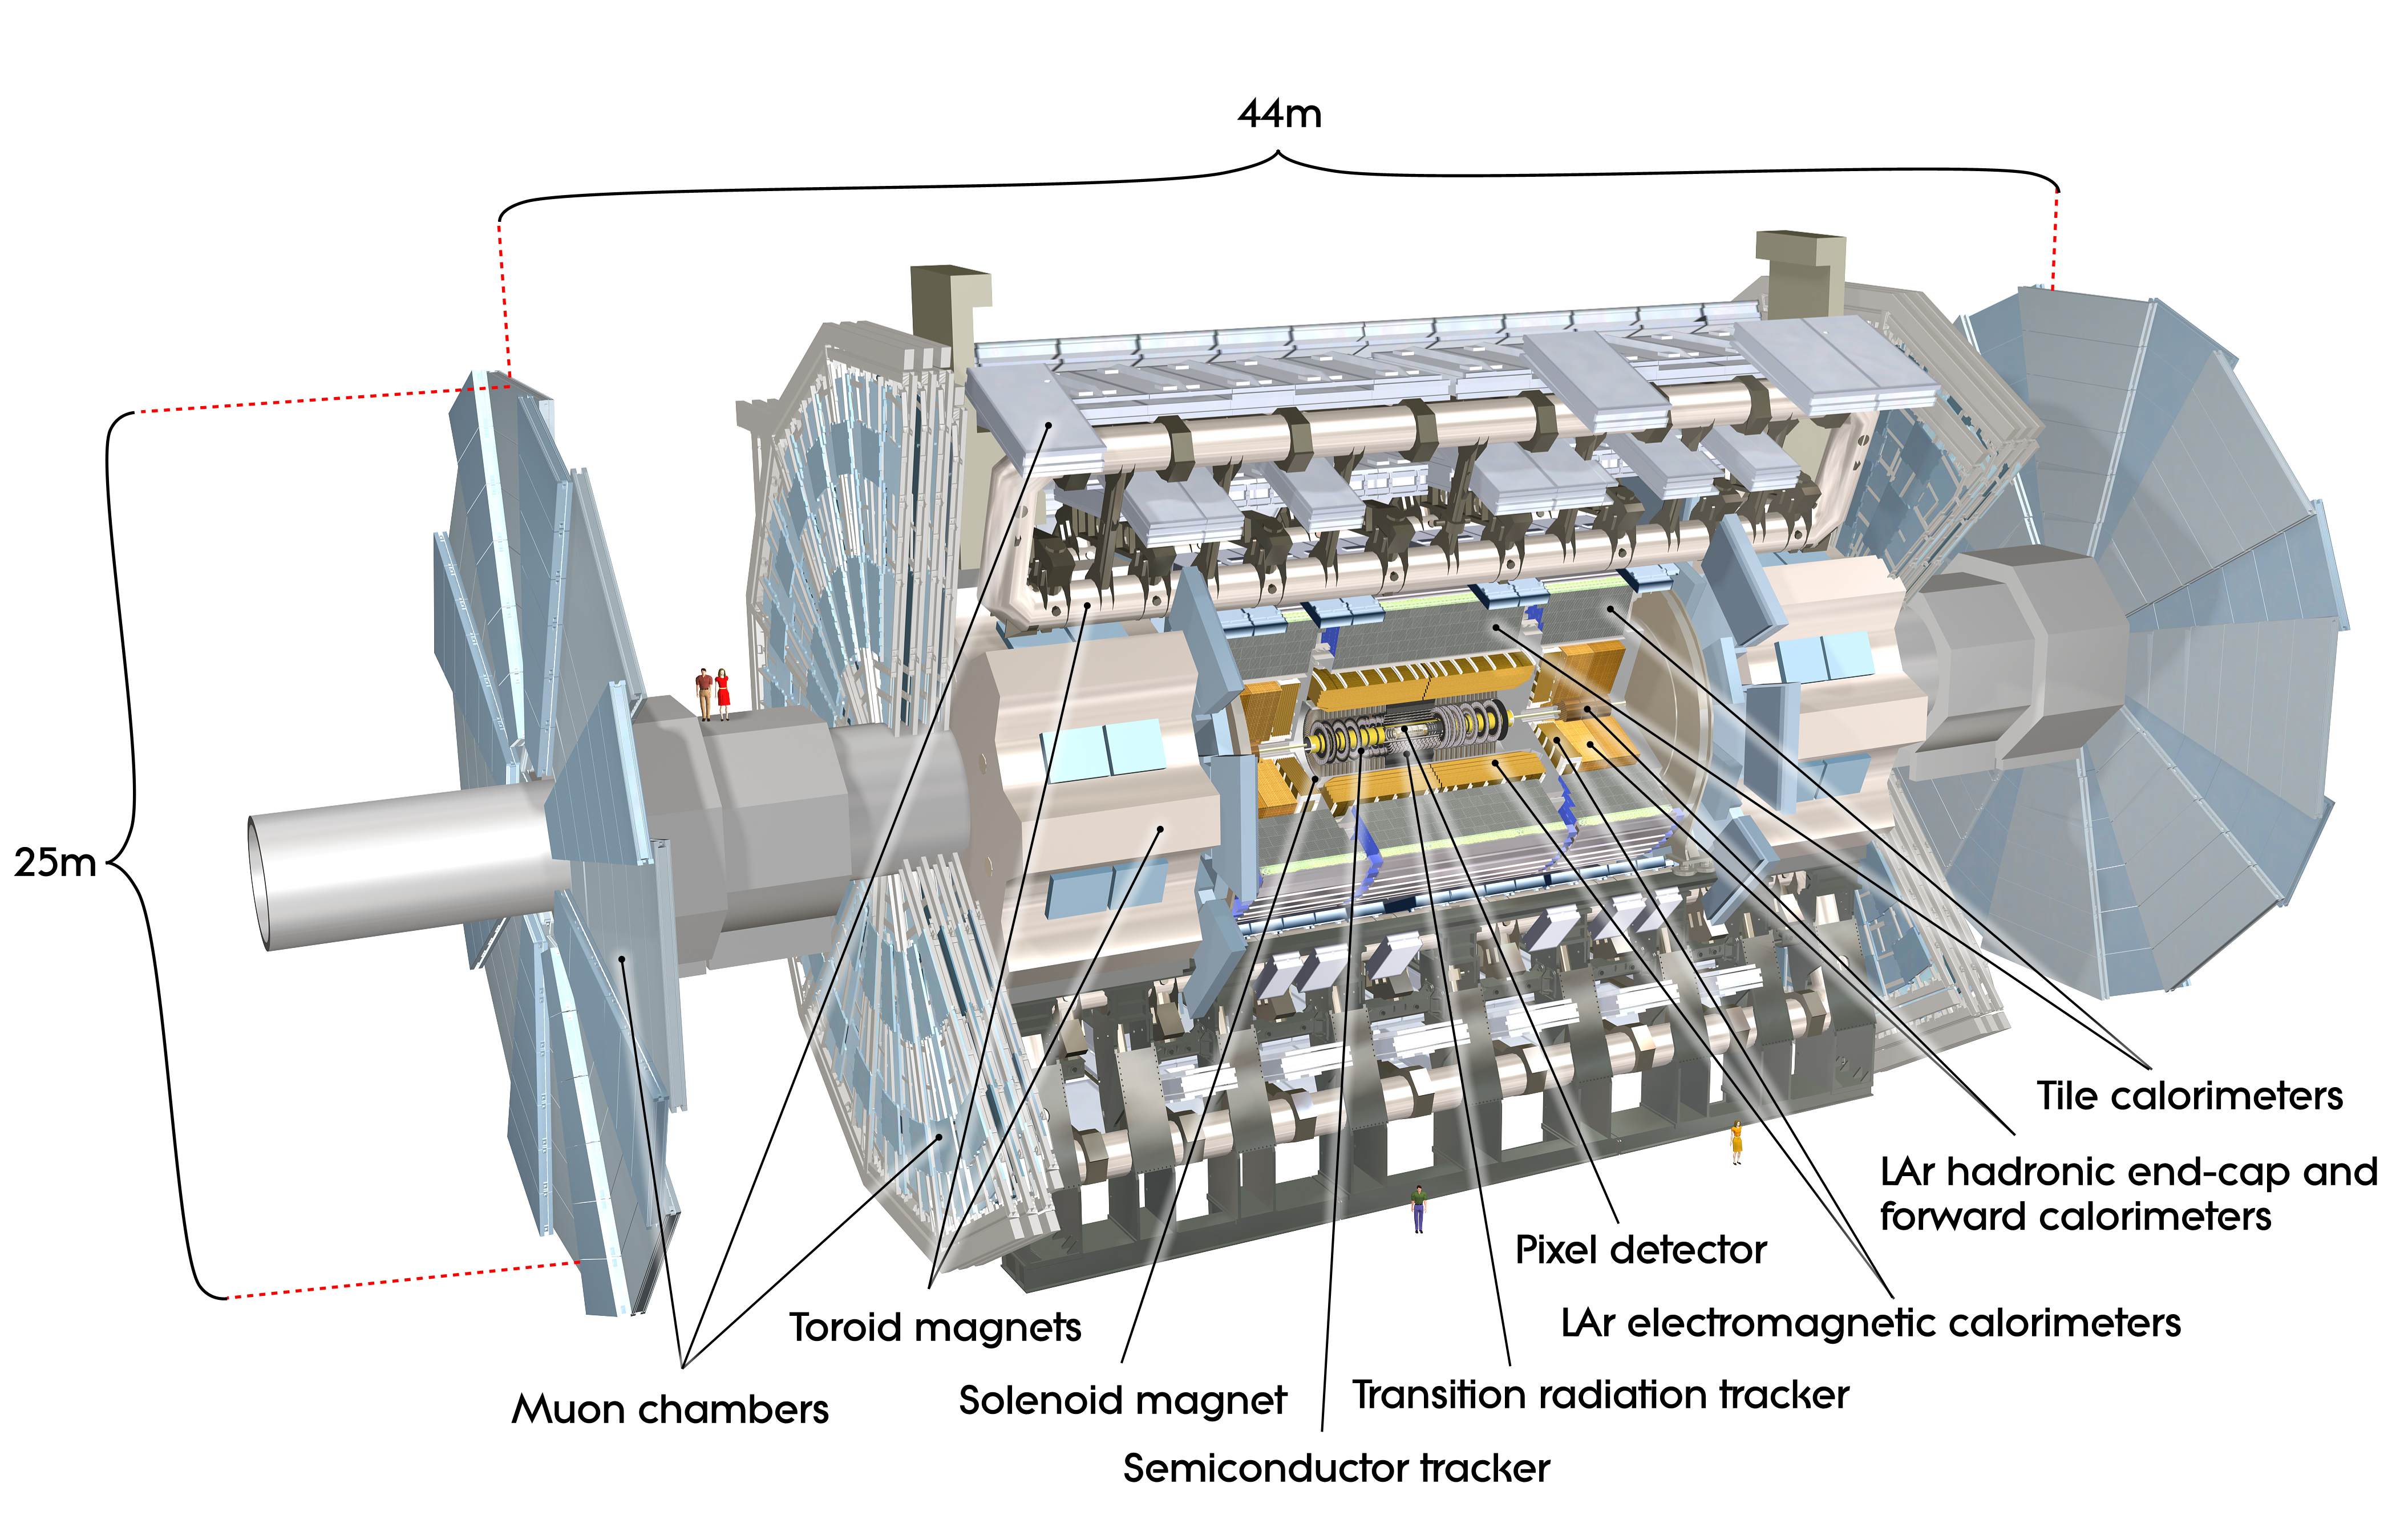
\includegraphics[width=0.90\textwidth]{figures/lhc-atlas/atlas-0803012_01.jpg}
  \caption{Scale rendering of the ATLAS detector with the various sub-detectors highlighted~\cite{atlas-cgi-detector}.}
  \label{fig:atlas-cartoon}
\end{figure}

\begin{figure}[tp]
  \centering
  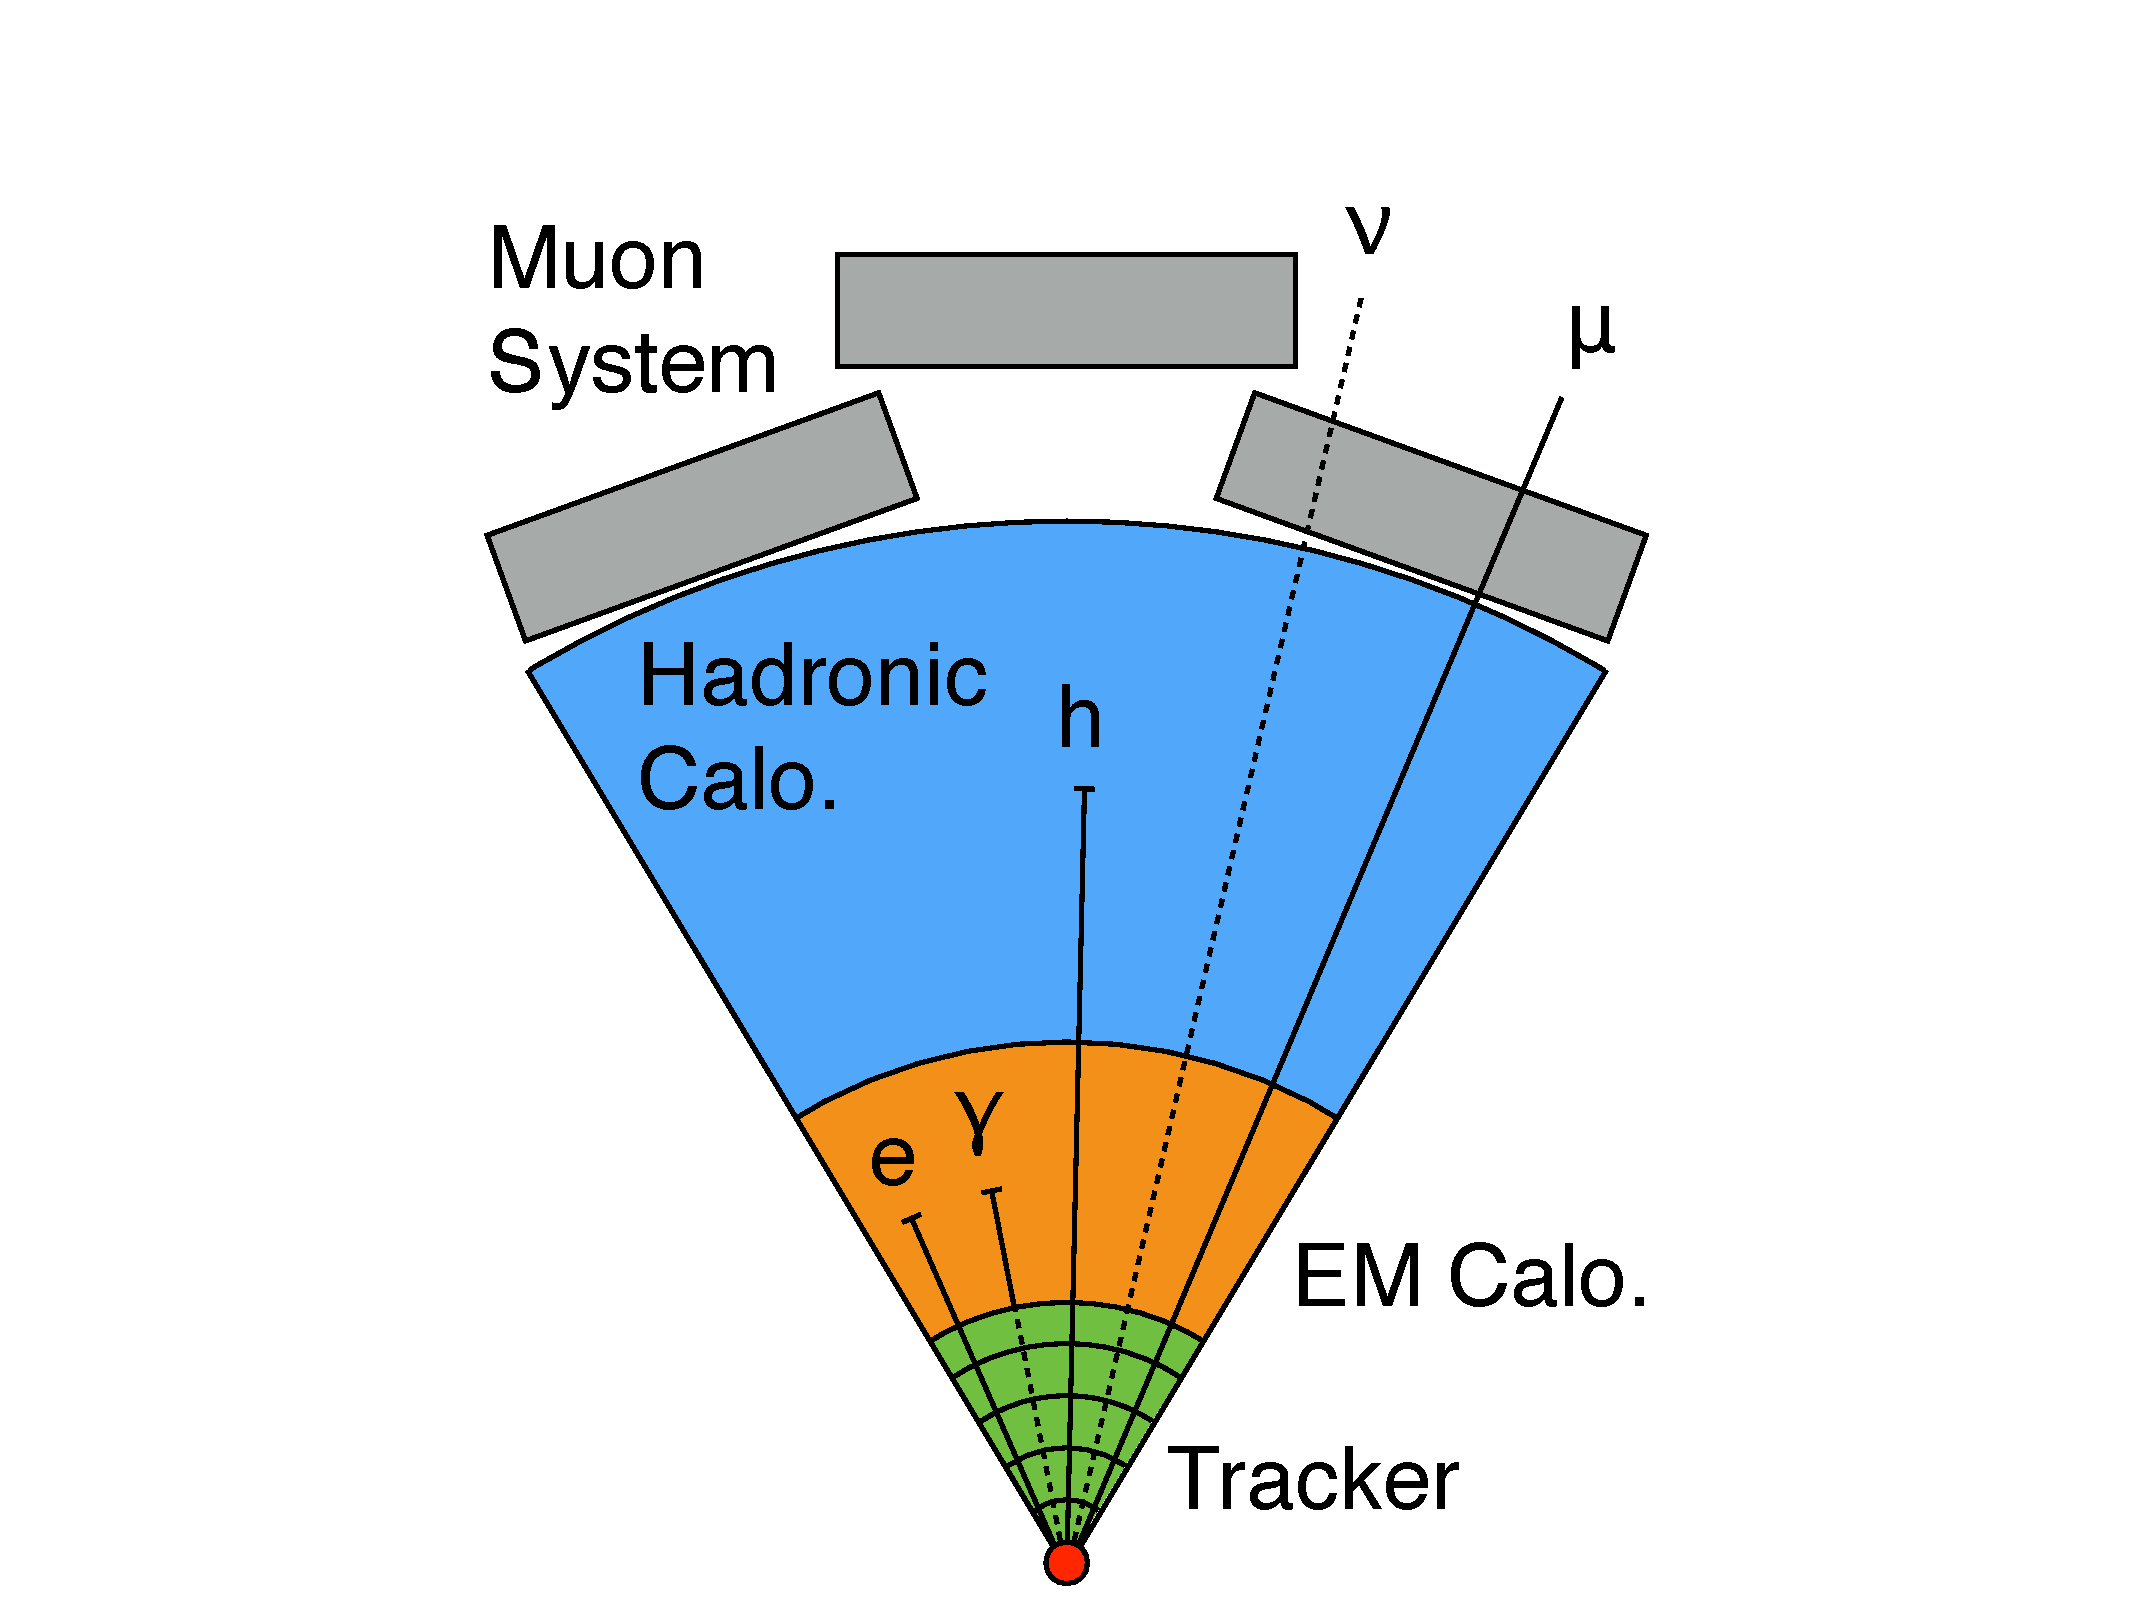
\includegraphics[width=0.5\textwidth]{figures/lhc-atlas/atlas-wedge-cartoon}
  \caption{Transverse schematic view of a wedge of the ATLAS detector. Charged particles leave tracks in the tracker, electrons and photons typically stop in the electromagnetic calorimeter, hadrons like charged pions typically stop in the hadronic calorimeter, and muons are tagged by the muon system as they exit. Neutrinos escape undetected.}
  \label{fig:atlas-wedge}
\end{figure}

\begin{figure}[tp]
  \centering
  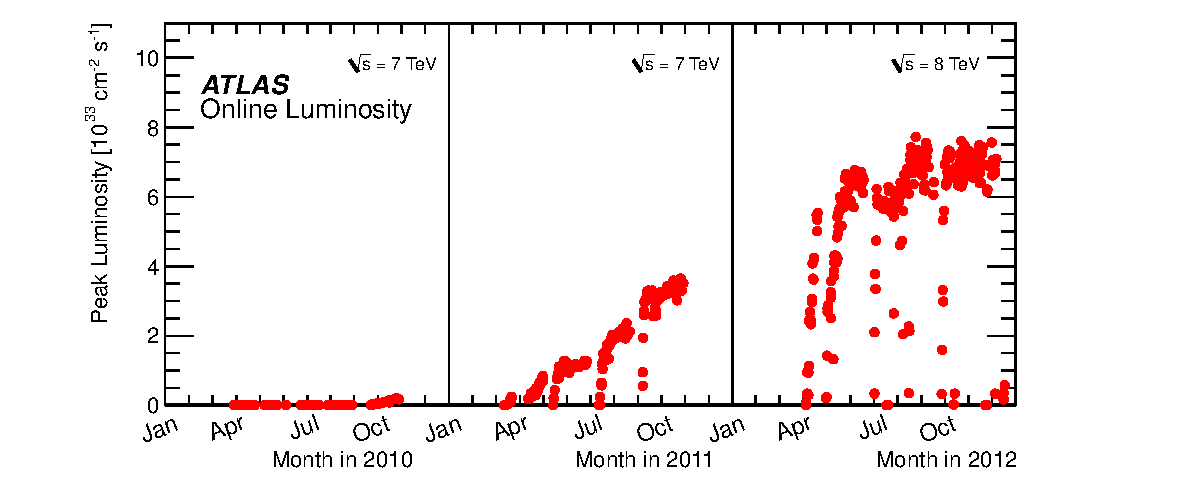
\includegraphics[width=0.90\textwidth]{figures/lhc-atlas/lumivstime}
  \caption{The peak ATLAS online luminosity as measured in different data-taking periods~\cite{atlas-lumi}. The peak Run-I luminosity is $0.8\times 10^{34} \text{cm}^{-2} \text{s}^{-1}$.}
  \label{fig:atlas-lumi-1}
\end{figure}

\begin{figure}[tp]
  \centering
  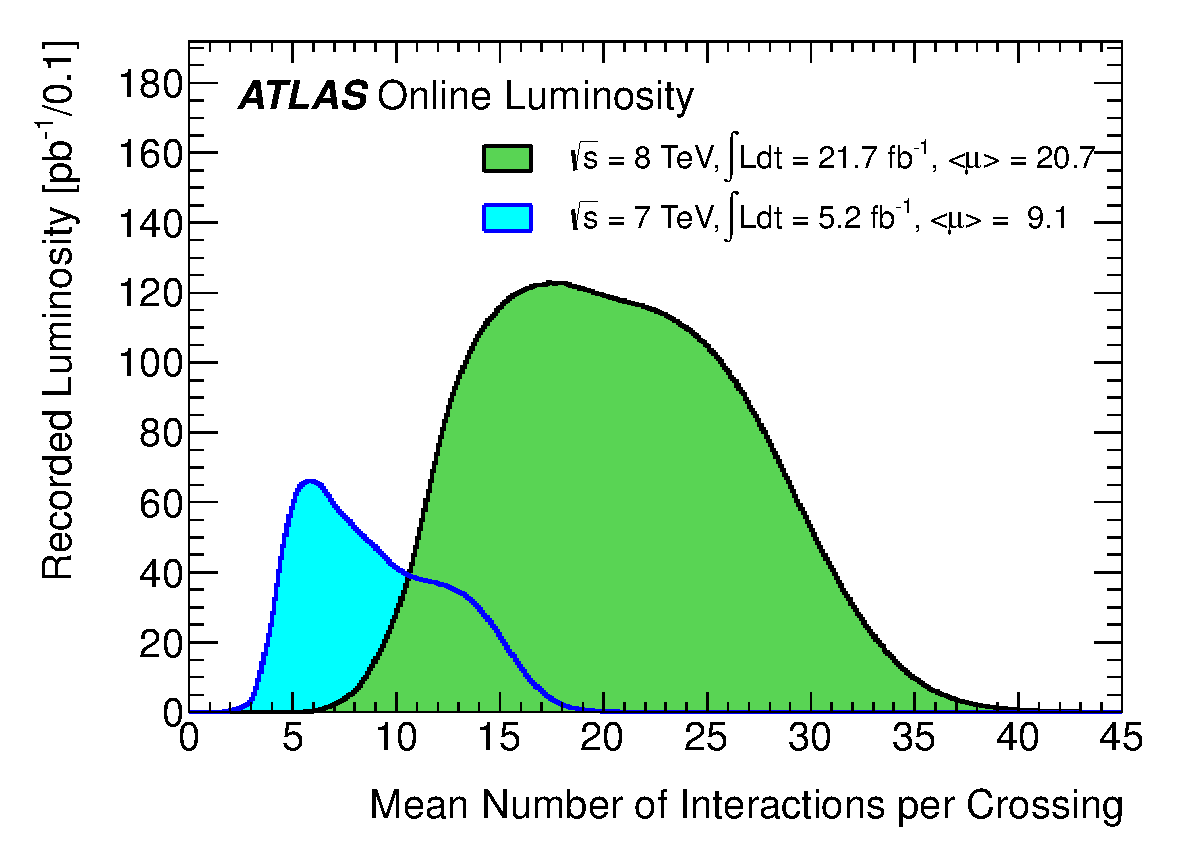
\includegraphics[width=0.48\textwidth]{figures/lhc-atlas/mu_2011_2012-dec}
  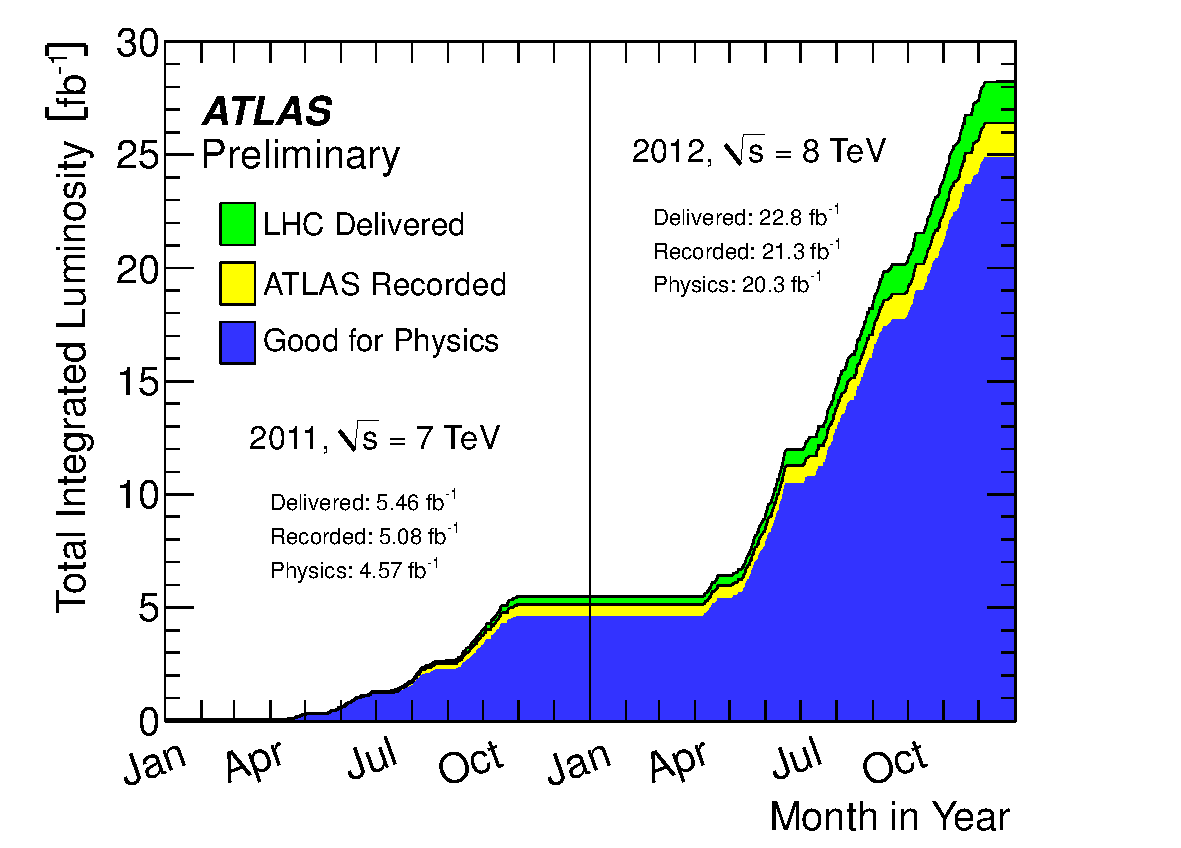
\includegraphics[width=0.48\textwidth]{figures/lhc-atlas/intlumivstime2011-2012DQ}
  \caption{Distributions of the recorded luminosity in bins of $\pileup$ (left) and the total integrated luminosity as a function of time (right)~\cite{atlas-lumi}. In 2011 (2012), the average $\pileup$ is 9.1 (20.7) and the total integrated luminosity for physics analysis is 4.6 $\ifb$. (20.3 $\ifb$).}
  \label{fig:atlas-lumi-2}
\end{figure}

\begin{figure}[tp]
  \centering
  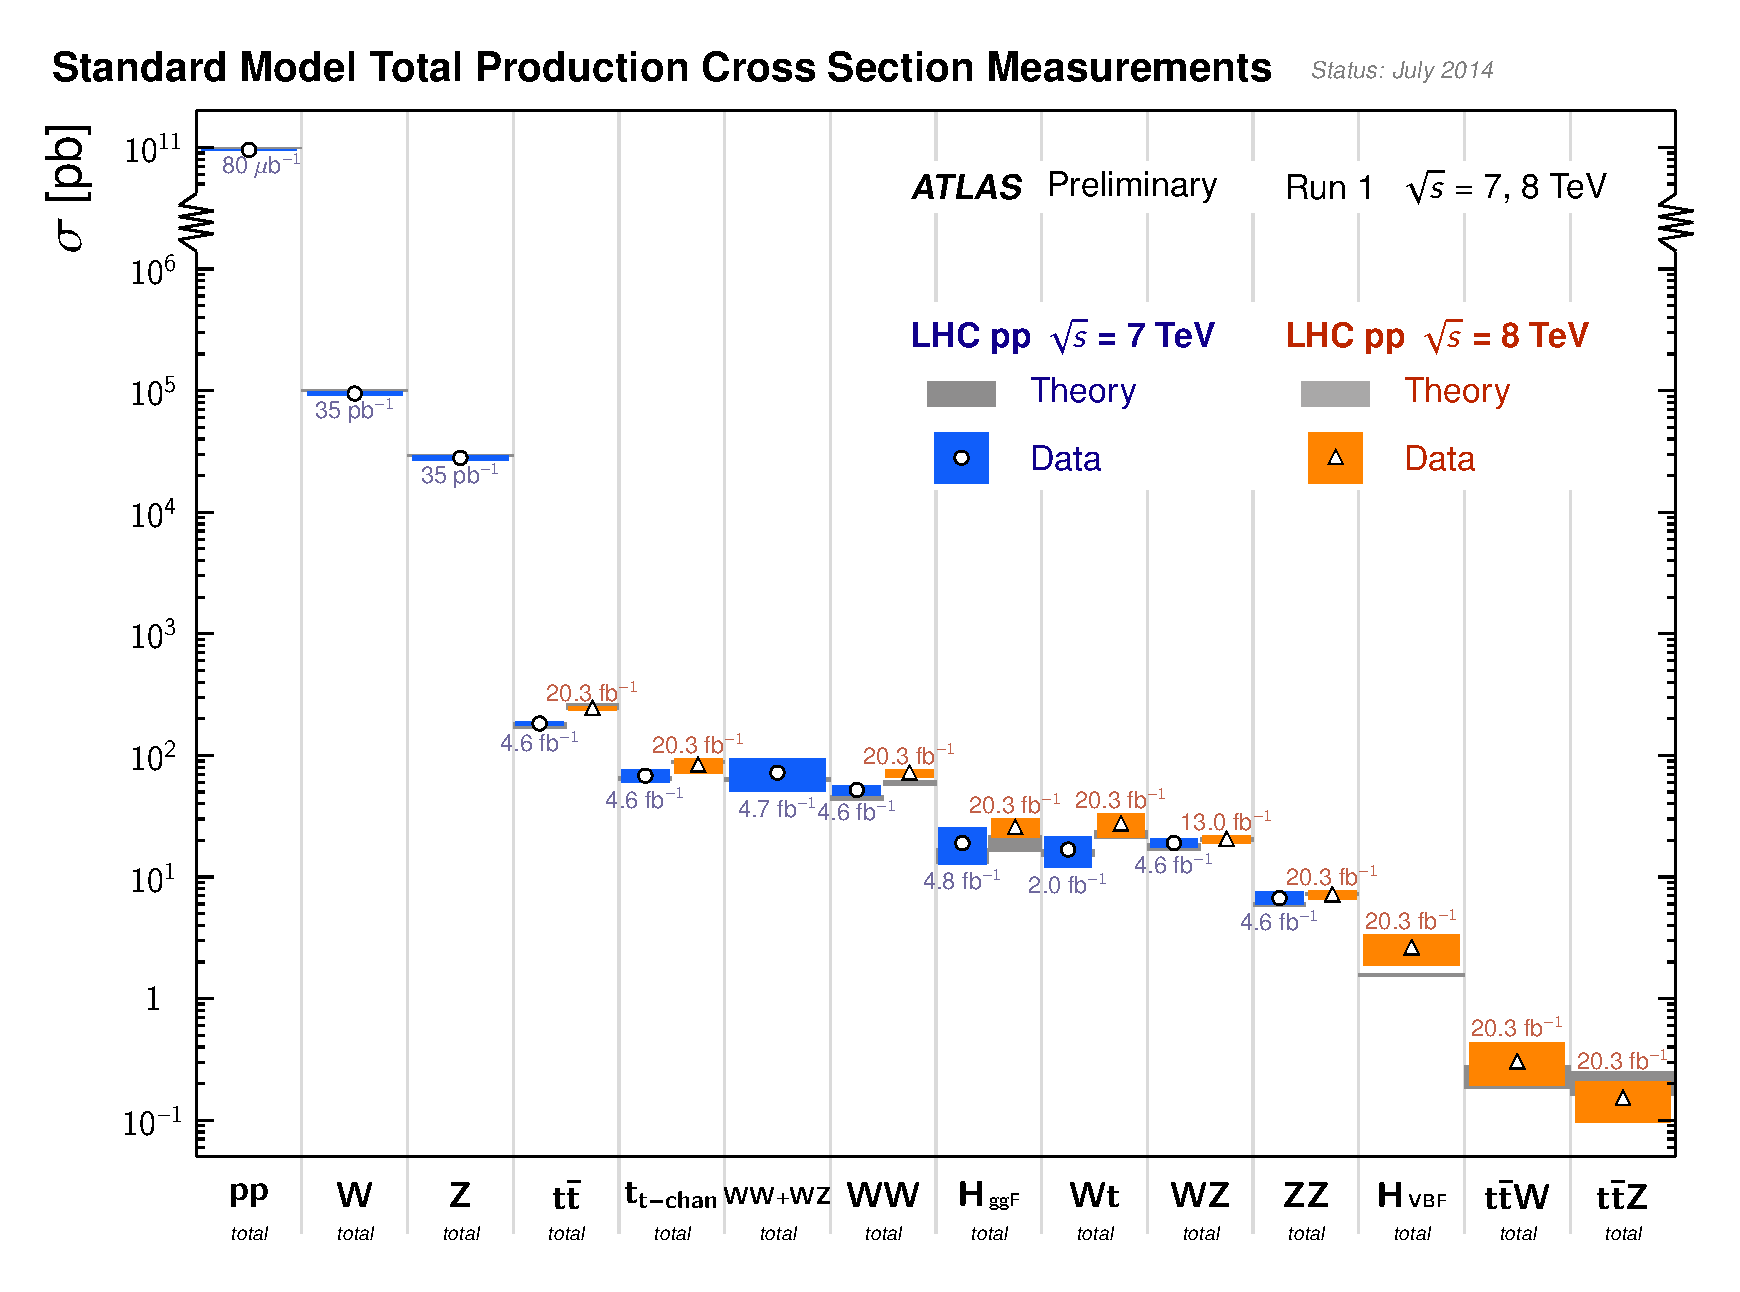
\includegraphics[width=0.90\textwidth]{figures/lhc-atlas/ATLAS_a_SMSummary_TotalXsect}
  \caption{Summary of cross sections measured at ATLAS in 7 and 8 TeV data-taking~\cite{2015.atlas-summary-SM}.}
  \label{fig:atlas-measurements}
\end{figure}

\subsection{Tracking}
\subsection{Calorimetry}
\subsection{Muon spectrometry}

\section{Particle identification}
\subsection{Muons}
\subsection{Electrons and photons}
\subsection{Hadrons}
% \subsubsection{Jets}
% \subsubsection{Jets from $b$-hadron decays}
\subsection{Neutrinos}
\section{Triggering}
\subsection{L1}
\subsection{HLT}

\begin{figure}[tp]
  \centering
  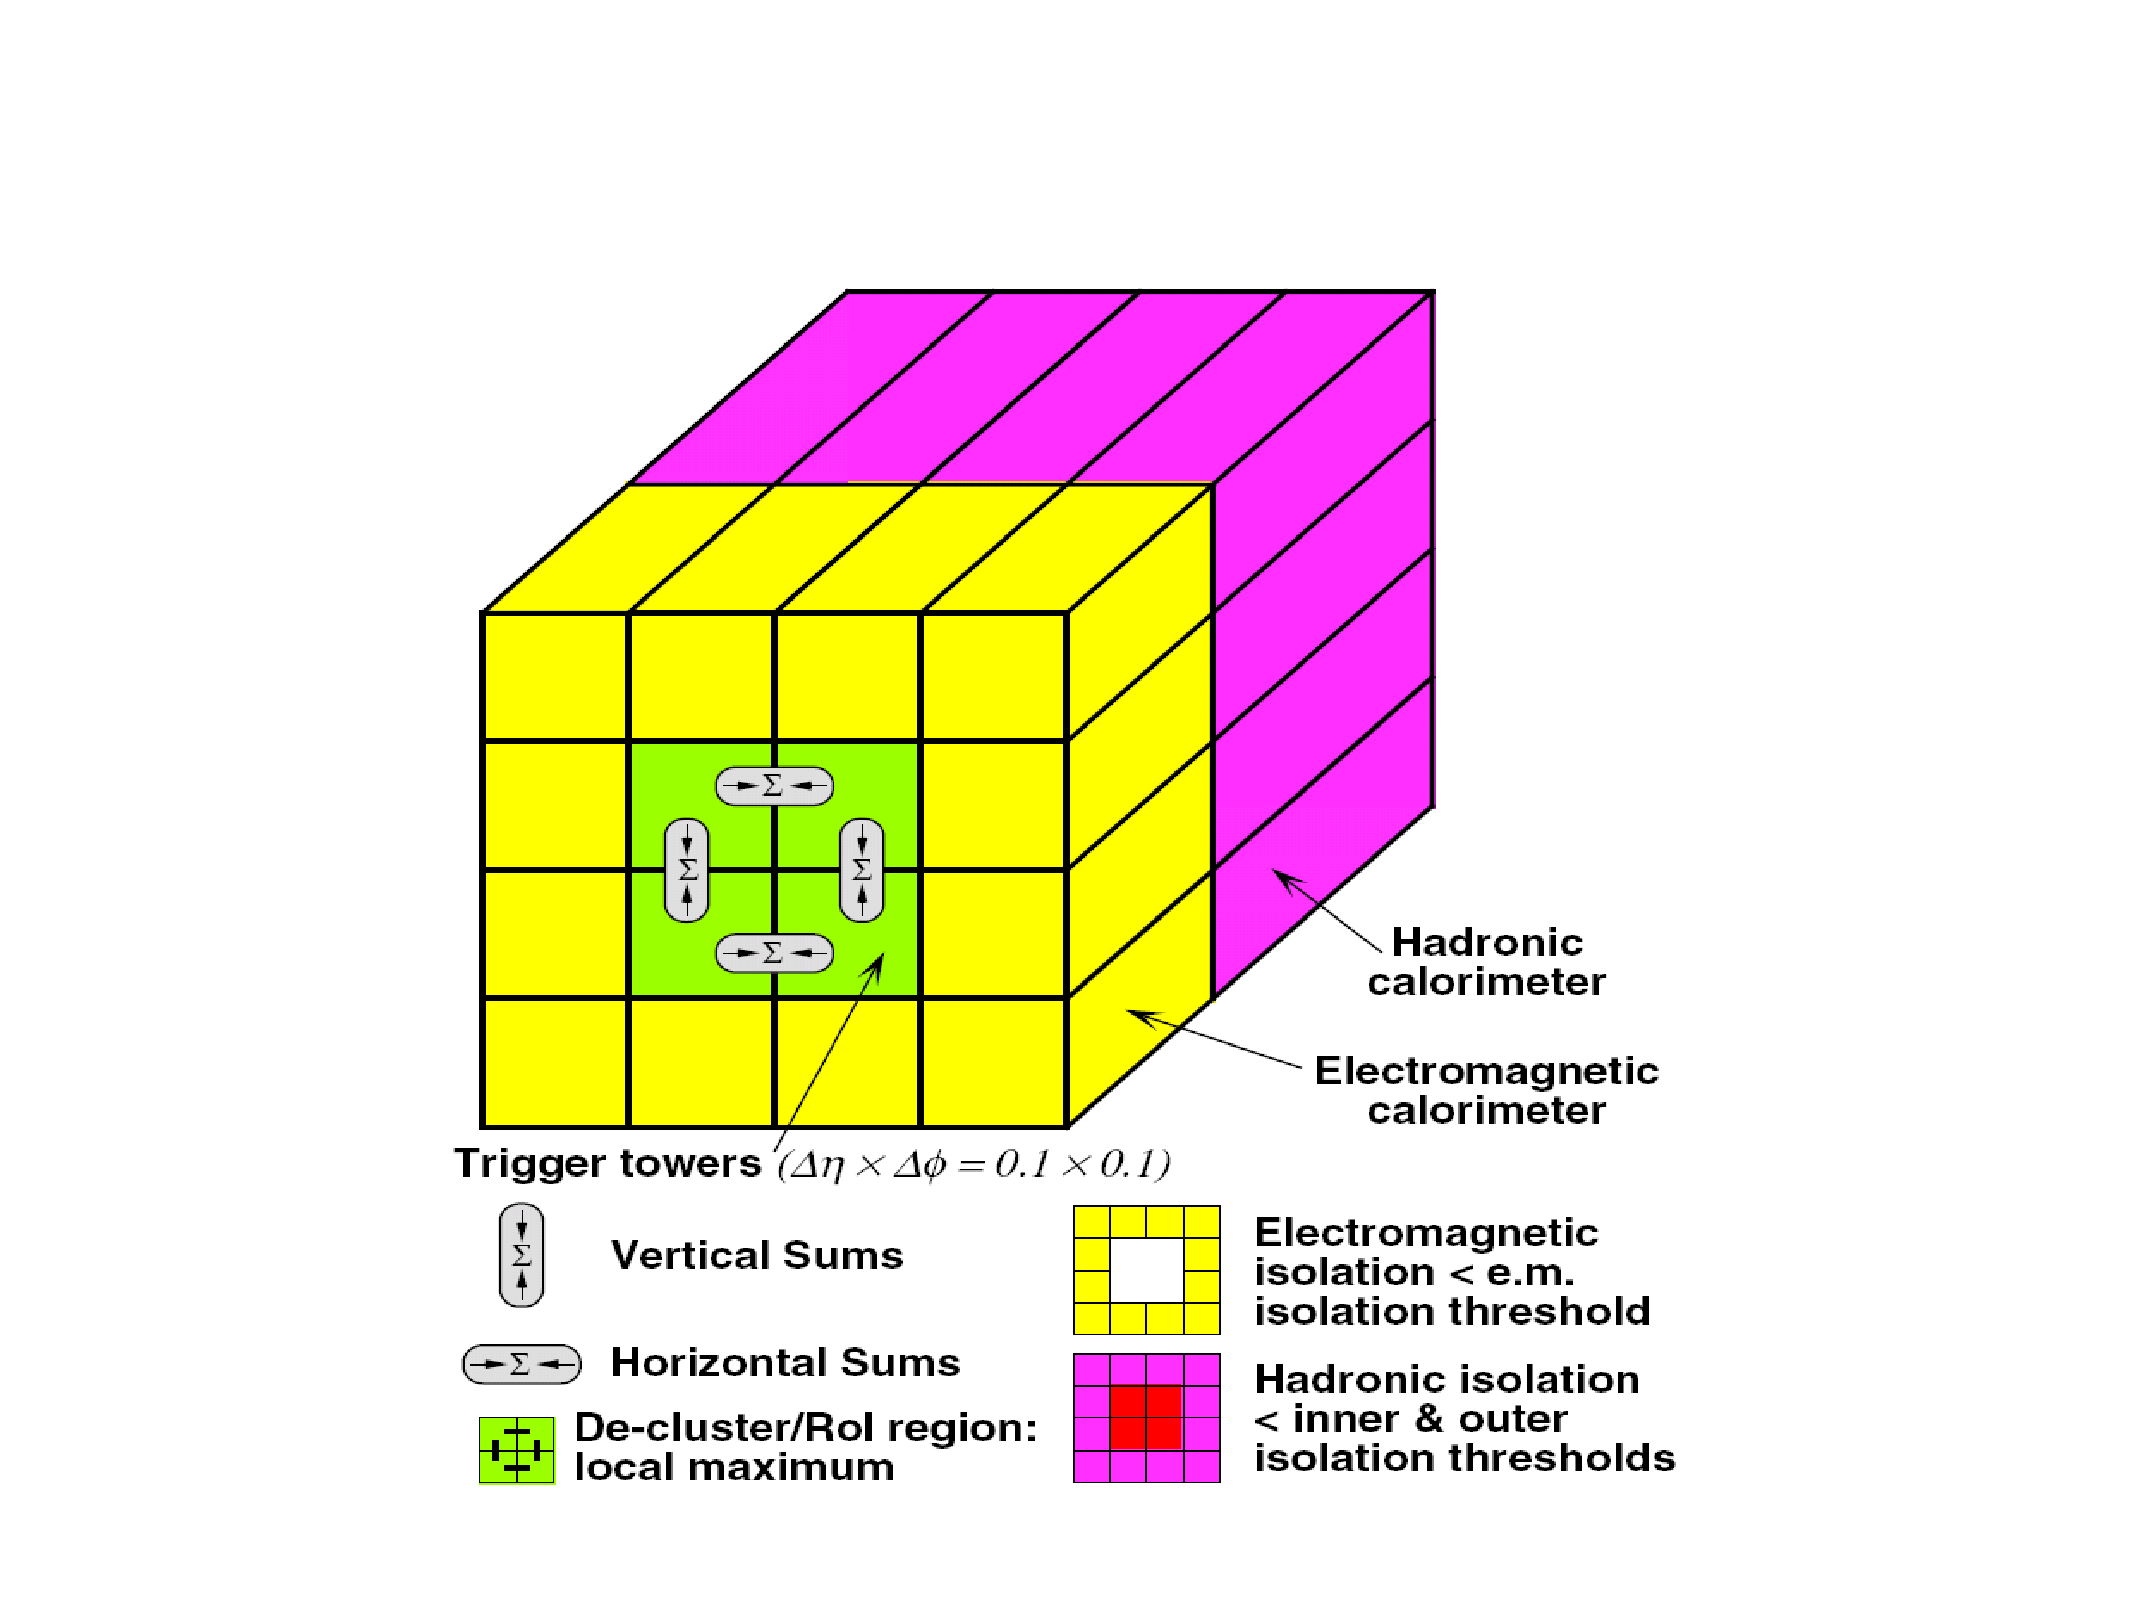
\includegraphics[width=0.80\textwidth]{figures/trigger/cartoonL1}
  \caption{Schematic view of the calorimeter granularity available at the L1 trigger~\cite{1998.ATLAS-TDR-L1}.}
  \label{fig:prospects-trigger-cartoonL1}
\end{figure}


